% !TEX root = RKWard_paper.tex
\section{Supplementary Figures}
\label{sec:Supplementary_figures}
This section gives additional figures for user interface elements and features of \pkg{RKWard}.

\begin{figure}[!h]
 \centering
 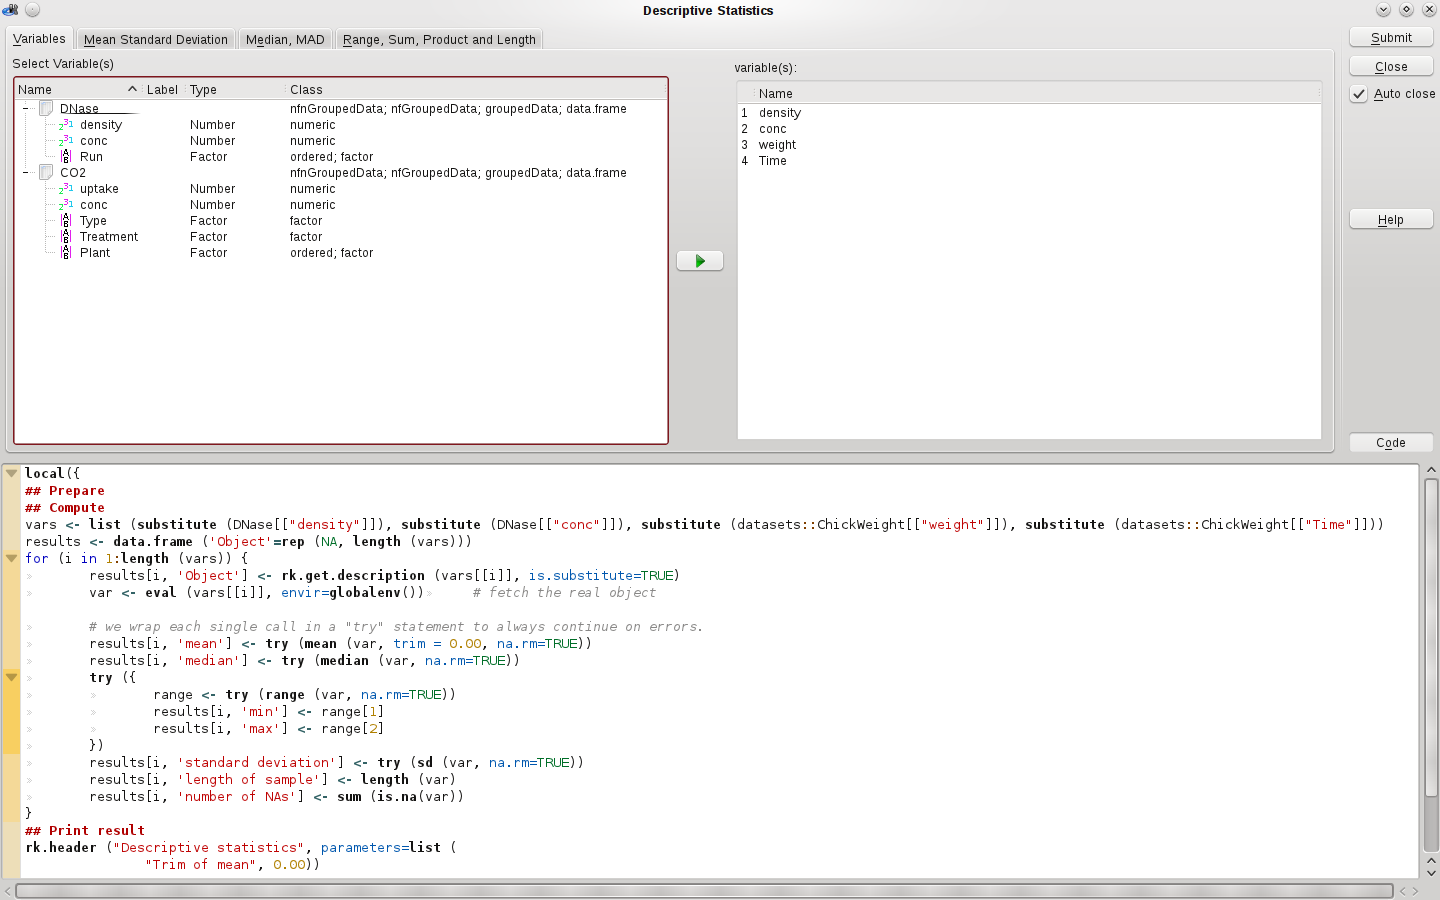
\includegraphics[width=15.4cm]{./figures/figure8_supplement.png}
 \caption{GUI dialog for sample contents of the output window (Figure 8 original paper). The syntax highlighted of the commands supports an easier reading of the code.
 \code{DNase} and \code{ChickWeight} data of the \pkg{datasets} packages were used.}
 \label{fig:figure8_supplement}
\end{figure}

\begin{figure}[!h]
 \centering
 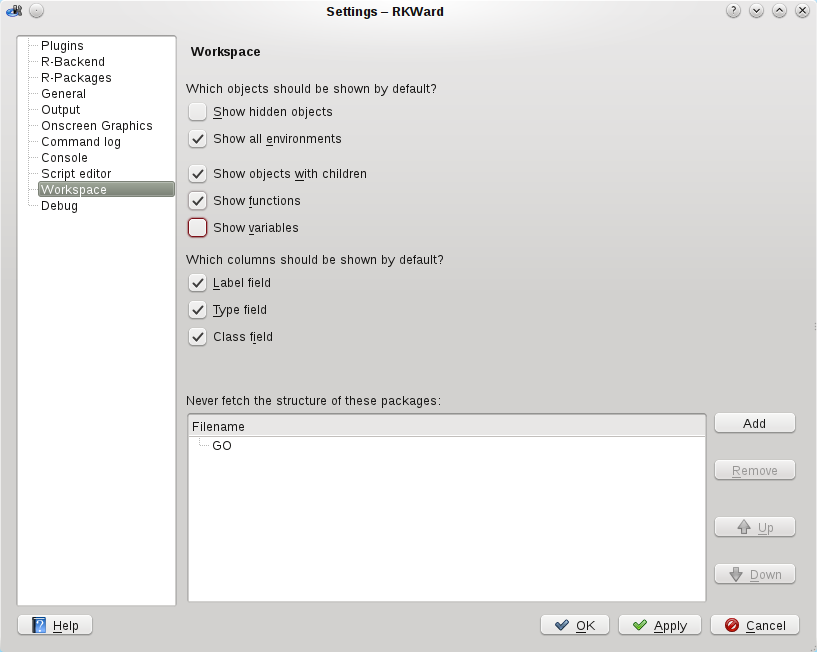
\includegraphics[width=15.4cm]{./figures/settings.png}
 \caption{GUI dialog for settings of details shown in \pkg{RKWard} (\texttt{Settings$\rightarrow$Configure RKWard$\rightarrow$Workspace}).}
 \label{fig:settings}
\end{figure}